\documentclass[11pt,a4paper]{article}

\usepackage[margin=0.8in]{geometry}
\usepackage{amsmath,amssymb}
\usepackage{graphicx}
\usepackage{booktabs}
\usepackage{float}
\usepackage{xcolor}
\usepackage{hyperref}
\usepackage{subcaption}
\usepackage{microtype}

\hypersetup{
    colorlinks=true,
    linkcolor=blue!70!black,
    urlcolor=blue!70!black,
    citecolor=blue!70!black
}
\graphicspath{{figures/}}

\title{\textbf{Flexibility versus Interpretability in High-Dimensional\\Multiclass Cancer Classification from RNA-Seq Data}}
\author{
    \textbf{Rajveer Vora} \qquad \textbf{Amartya Amritanshu} \qquad \textbf{P.\ Sanjith Reddy} \\[0.6em]
    Indian Statistical Institute, Kolkata \\[0.25em]
    \small Course Project: Regression Techniques \\[0.35em]
    \small \href{https://github.com/RajveerVoraUni/gene-expression-cancer}{\textbf{GitHub Repository}}
}
\date{September--November 2026}

\begin{document}

\maketitle

\begin{abstract}
In high-dimensional transcriptomic cancer classification ($p \gg n$), strong biological signals across tissue lineages cause standard machine learning models to reach an apparent performance ceiling. Consequently, raw classification accuracy provides limited insight into clinical viability. In this study, we investigate the trade-offs between model flexibility, feature parsimony, biomarker stability, and probability calibration across regularized linear models, tree ensembles, and neural networks on the TCGA Pan-Cancer RNA-Seq dataset. We demonstrate that Elastic Net logistic regression achieves the optimal clinical trade-off: matching the predictive accuracy of complex black-box architectures while isolating a compact, reproducible gene panel. In contrast, tree ensembles suffer from severe feature selection instability caused by transcriptomic collinearity. Furthermore, under extreme sample scarcity, regularized linear models generalize robustly due to strong inductive bias, whereas gradient-boosted trees degrade. Our findings indicate that for clinical transcriptomic assays, sparse regularized linear models dominate complex architectures in interpretability, stability, and sample efficiency.
\end{abstract}

\section{Introduction and Problem Formulation}

High-throughput RNA sequencing (RNA-Seq) enables comprehensive profiling of cellular transcriptomes, providing continuous expression measurements for tens of thousands of genes per biological specimen. In precision oncology, identifying the primary anatomical site of origin for solid tumors is fundamental for clinical decision-making. Histopathological examination and immunohistochemistry (IHC) are standard, yet approximately 3\% to 5\% of all malignant neoplasms present as Cancer of Unknown Primary (CUP)~\cite{weinstein2013cancer}. In metastatic presentations where biopsy material is scarce or poorly differentiated, bulk transcriptomic profiling offers an objective, automated path toward determining primary lineage and guiding targeted therapies.

However, machine learning applied to bulk RNA-Seq is characterized by the severe $p \gg n$ curse of dimensionality: while tens of thousands of genes ($p = 20{,}531$) are simultaneously quantified, patient cohorts typically number in the hundreds ($n = 801$). In this underdetermined statistical regime, several profound challenges arise:
\begin{enumerate}
    \item \textbf{The Performance Ceiling Effect:} Lineage-specific differentiation programs produce immense expression differentials between distinct anatomical organs (e.g., renal tubular cells versus mammary epithelium). As a result, nearly all contemporary classifiers—whether simple linear models or multi-layer neural networks—readily attain $\ge 98\%$ test accuracy. Evaluating models solely through top-level accuracy yields an uninformative performance ceiling that fails to differentiate clinical utility.
    \item \textbf{Transcriptomic Collinearity and Gene Co-Regulation:} Genes do not function as independent statistical variables; rather, they operate within concerted biological pathways, co-regulated by shared transcription factors and epigenetic chromatin complexes. Consequently, thousands of genes exhibit pairwise Pearson correlations exceeding $r > 0.85$. Under such extreme collinearity, variable-selection algorithms may select arbitrary individual gene representatives from co-regulated modules, leading to unstable biomarker panels across slightly perturbed patient cohorts.
    \item \textbf{Clinical Parsimony versus Sequencing Cost:} While research sequencing quantifies all $20{,}000+$ transcripts, deploying a whole-transcriptome assay in frontline clinical diagnostics is economically and operationally prohibitive. Developing targeted assays (such as quantitative RT-PCR or NanoString panels like Oncotype DX or MammaPrint) requires isolating a parsimonious, robust subset of under 250 genes without sacrificing diagnostic reliability.
    \item \textbf{Risk of Experimental Data Leakage:} High-dimensional feature selection and standard scaling are notoriously vulnerable to data snooping. Applying unsupervised variance filtering or normalization across the entire dataset prior to splitting leaks test distribution information, producing overly optimistic, non-reproducible performance claims.
\end{enumerate}

To address these core challenges, this benchmark departs from standard accuracy chasing to systematically examine three fundamental research questions:
\begin{itemize}
    \item \textbf{Q1 (Flexibility vs. Performance):} Does transitioning from linear classifiers to non-linear tree ensembles and deep neural networks provide measurable predictive gains in the transcriptomic $p \gg n$ regime?
    \item \textbf{Q2 (Feature Selection Stability):} How consistent and biologically reproducible are the gene signatures identified by sparse linear regularizers compared to tree-based split importances across independent patient resamples?
    \item \textbf{Q3 (Sample Efficiency):} How do distinct model families degrade when clinical training data is severely starved ($n_{\text{train}} \to 30$)?
\end{itemize}

\section{Exploratory Data Analysis and Biological Insights}

This study benchmarks models using the UCI TCGA Pan-Cancer RNA-Seq dataset~\cite{fiorini2016gene,weinstein2013cancer}, containing $n = 801$ primary solid tumor samples with $p = 20{,}531$ continuous Illumina HiSeq gene expression values ($\log_2(\text{RSEM} + 1)$ normalized).

\subsection{Tumor Cohorts and Quality Control}
The dataset encompasses five primary solid tumor types representing major adult malignancies:
\begin{itemize}
    \item \textbf{BRCA (Breast Invasive Carcinoma, $n = 300$, 37.5\%):} The largest cohort, characterized by luminal and basal epithelial oncogenic signaling (e.g., estrogen receptor and HER2 pathways).
    \item \textbf{KIRC (Kidney Renal Clear Cell Carcinoma, $n = 146$, 18.2\%):} Arises from renal proximal tubular epithelium, dominated by VHL mutations and hypoxia-inducible pathway overexpression.
    \item \textbf{LUAD (Lung Adenocarcinoma, $n = 141$, 17.6\%):} Non-small cell lung malignancy originating in alveolar glandular tissue, marked by surfactant protein expression and RTK/RAS alterations.
    \item \textbf{PRAD (Prostate Adenocarcinoma, $n = 136$, 17.0\%):} Glandular prostate carcinoma driven by androgen receptor transcriptional networks and prostate-specific kallikreins.
    \item \textbf{COAD (Colon Adenocarcinoma, $n = 78$, 9.7\%):} Colorectal epithelial cancer dominated by Wnt/$\beta$-catenin signaling and gut-specific cytokeratins.
\end{itemize}

The resulting class imbalance ratio of approximately $3.8:1$ (Figure~\ref{fig:class-balance}) necessitates the use of stratified train/test sampling and macro-averaged metrics (Macro-F1) alongside multi-class cross-entropy log-loss. 

Quality control analysis across sample-level mean expression and zero-fraction (Figure~\ref{fig:sample-qc}) reveals consistent distributions across all five tumor classes: median mean expression ranges narrowly between $6.28$ and $6.54$, and median zero-count fractions range from $0.136$ to $0.155$. This uniformity confirms the absence of technical artifacts, severe batch effects, or anomalous library preparation failures across patient specimens.

\begin{figure}[H]
    \centering
    \begin{subfigure}[b]{0.48\textwidth}
        \centering
        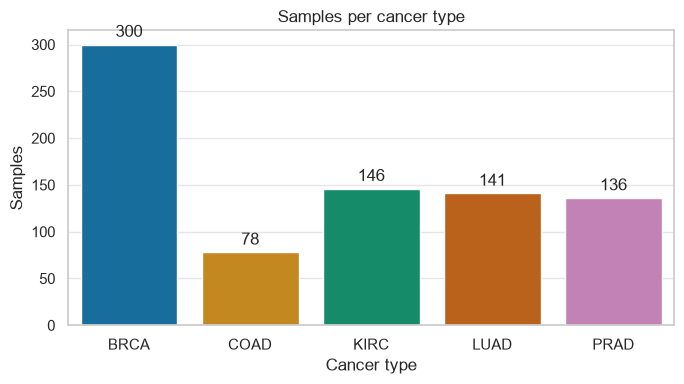
\includegraphics[width=\textwidth]{01_class_balance.png}
        \caption{Patient sample distribution across tumor types.}
        \label{fig:class-balance}
    \end{subfigure}
    \hfill
    \begin{subfigure}[b]{0.48\textwidth}
        \centering
        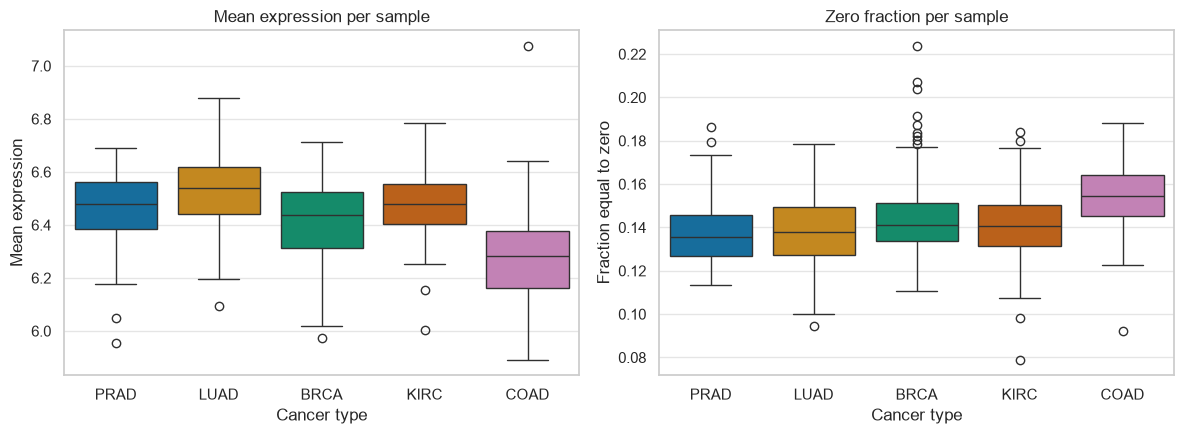
\includegraphics[width=\textwidth]{02_sample_qc_by_class.png}
        \caption{Sample-level mean expression and zero fraction.}
        \label{fig:sample-qc}
    \end{subfigure}
    \caption{Dataset composition and sample-level quality control summaries.}
\end{figure}

\subsection{Dimensionality, Variance Dispersion, and Latent Structure}
A fundamental characteristic of transcriptomic profiling is that a vast majority of the $20{,}531$ genes represent basic cellular housekeeping transcripts (e.g., ribosomal, mitochondrial, and metabolic structural genes) with near-uniform expression across tissues. As shown in the gene mean-variance dispersion plot (Figure~\ref{fig:mean-var}), variance is heavily concentrated in a small minority of features: only the top $5\%$ to $10\%$ of genes exhibit substantial across-patient variation, providing an empirical basis for unsupervised variance filtering as a preliminary dimensionality reduction step.

\begin{figure}[H]
    \centering
    \begin{subfigure}[b]{0.48\textwidth}
        \centering
        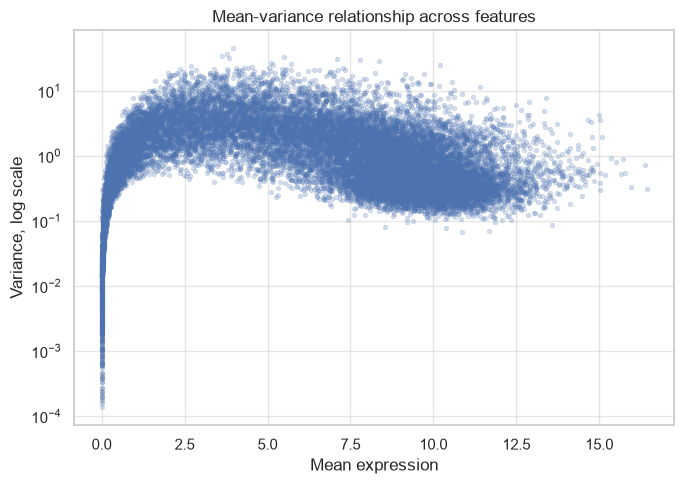
\includegraphics[width=\textwidth]{03_gene_mean_variance.png}
        \caption{Gene mean vs. variance relationship.}
        \label{fig:mean-var}
    \end{subfigure}
    \hfill
    \begin{subfigure}[b]{0.48\textwidth}
        \centering
        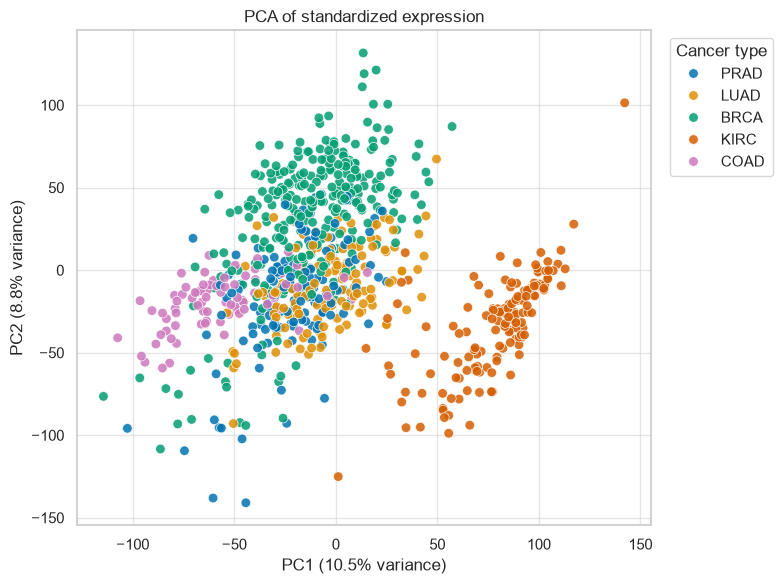
\includegraphics[width=\textwidth]{05_pca_pc1_pc2.png}
        \caption{Unsupervised PCA (PC1 vs. PC2).}
        \label{fig:pca-scatter}
    \end{subfigure}
    \caption{Feature distribution and latent cluster structure.}
\end{figure}

Unsupervised Principal Component Analysis (PCA) performed on standardized expression data confirms that approximately $200$ to $250$ principal components capture over $85\%$ of cumulative variance. More strikingly, a two-dimensional projection onto the first two principal components (PC1 and PC2, Figure~\ref{fig:pca-scatter}) already produces distinct, well-separated clusters corresponding to each tumor type without access to class labels. This unsupervised separation indicates that tissue-of-origin differentiation programs constitute the primary axes of biological variance in the human transcriptome. 

A hierarchical clustered heatmap of the 50 most variable genes (Figure~\ref{fig:heatmap}) confirms the existence of sharp, block-diagonal transcriptomic signatures uniquely upregulated within each cancer type. This pronounced linear separability provides a clear mathematical explanation for why standard linear classifiers achieve exceptionally high diagnostic accuracy.

\begin{figure}[H]
    \centering
    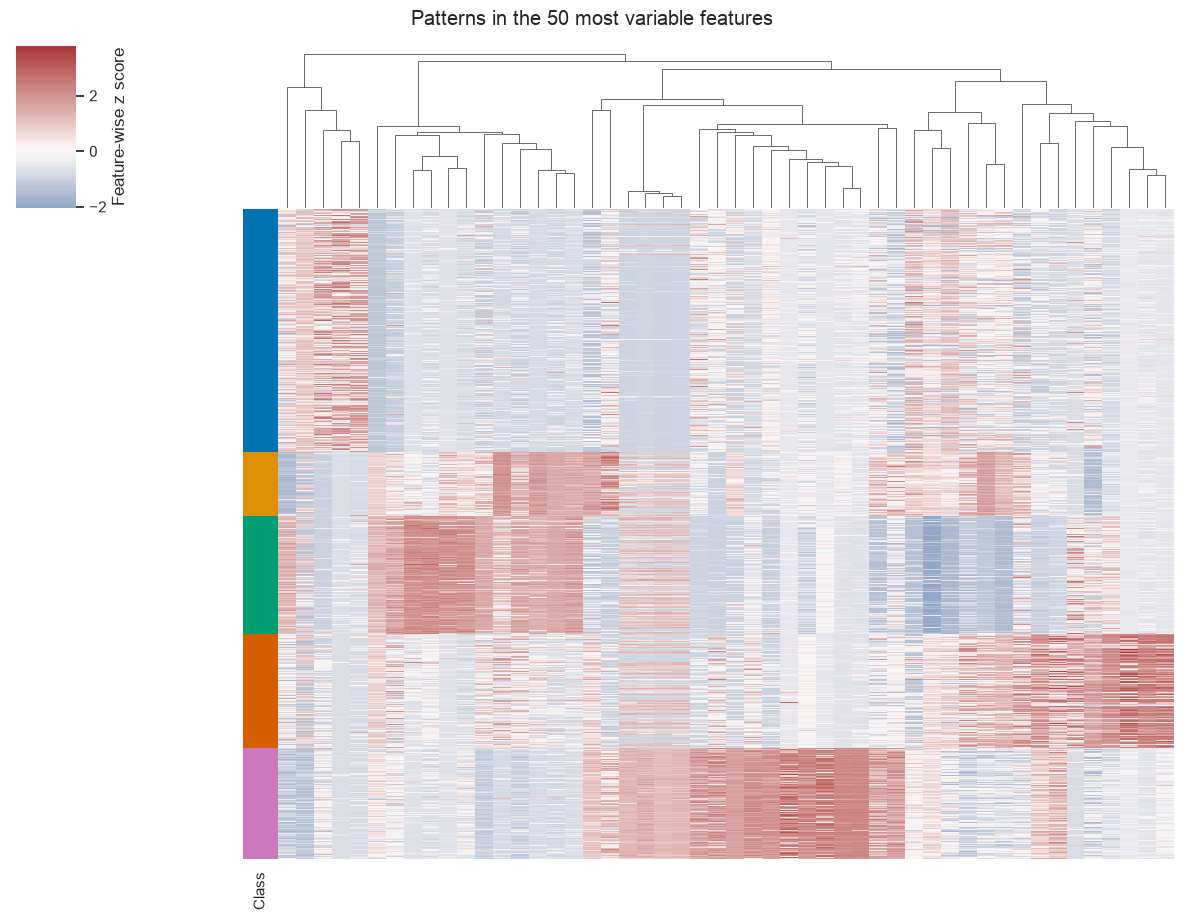
\includegraphics[width=0.75\textwidth]{06_top_variable_feature_heatmap.png}
    \caption{Clustered heatmap of standardized expression for the 50 most variable genes, grouped by tumor type.}
    \label{fig:heatmap}
\end{figure}

\section{Experimental Methodology}

\subsection{Leakage-Free Resampling Protocol}
Data leakage is a well-documented source of irreproducibility in genomic machine learning. When feature selection, centering, or scaling utilizes statistics computed across the entire cohort, information from test specimens inadvertently contaminates the training phase. 

To guarantee strict statistical isolation, we enforce a leak-free evaluation protocol:
\begin{enumerate}
    \item \textbf{Frozen Outer Splits:} The dataset is partitioned into $N = 10$ repeated stratified 80/20 train/test splits ($N_{\text{train}} = 640, N_{\text{test}} = 161$) using fixed seeds. The test fold of each split is placed in cold storage and remains strictly untouched during all feature processing and training.
    \item \textbf{Training-Only Transformations:} Within each split, gene variance ranking, selection of the top $p = 1{,}000$ genes, standard scaling ($\mu_{\text{train}}, \sigma_{\text{train}}$), and PCA projection matrices ($V_k$) are calculated strictly using the $640$ training samples. The learned parameters are then applied deterministically to transform the corresponding test fold.
\end{enumerate}

\subsection{Model Formulation and Theoretical Contrast}
We evaluate eight models spanning three distinct architectural paradigms, selected to contrast linear, tree-based, and deep neural learning under extreme collinearity:
\begin{enumerate}
    \item \textbf{Unpenalized Multinomial Logistic Regression (Softmax):} Baseline linear model modeling class probabilities via the softmax link function:
    \begin{equation}
        P(Y = c \mid x) = \frac{\exp(w_c^T x + b_c)}{\sum_{j=1}^C \exp(w_j^T x + b_j)}
    \end{equation}
    optimizing multi-class cross-entropy via L-BFGS with no regularizing constraint.
    \item \textbf{Ridge Logistic Regression ($L_2$):} Adds an isotropic quadratic penalty $\frac{1}{2}\lambda \|\beta\|_2^2$ to the log-likelihood. While Ridge shrinks all coefficients proportionally toward zero to stabilize matrix inversion in collinear spaces, it retains all $1{,}000$ features, offering zero model parsimony.
    \item \textbf{Lasso Logistic Regression ($L_1$):} Introduces a non-smooth $L_1$ penalty $\lambda \|\beta\|_1$~\cite{tibshirani1996regression}. Geometrically, the sharp corners of the $L_1$ polytope force small coefficients to exact numerical zeros via the SAGA proximal solver, yielding an ultra-sparse, interpretable gene panel. However, under high transcriptomic collinearity, Lasso arbitrarily selects one gene from a co-regulated cluster and suppresses the remainder.
    \item \textbf{Elastic Net Logistic Regression ($L_1 + L_2$):} Bridges Lasso and Ridge through a convex combination of penalties~\cite{zou2005regularization}:
    \begin{equation}
        \Omega(\beta) = \lambda \left[ \alpha \|\beta\|_1 + \frac{1 - \alpha}{2} \|\beta\|_2^2 \right]
    \end{equation}
    where $\alpha \in [0, 1]$ controls the sparsity ratio. The strictly convex quadratic term enforces the \emph{grouping property}: highly correlated genes receive similar weights and are retained together in the active biomarker set, stabilizing selection across patient cohorts.
    \item \textbf{Random Forest:} Non-linear ensemble of 200 deep decision trees ($d = 32$) trained via bootstrap aggregation (bagging) and randomized feature subsampling ($\sqrt{p}$). While resilient to outliers, greedy axis-aligned recursive partitioning amidst thousands of correlated genes creates high stochastic variance in split choice.
    \item \textbf{XGBoost (Histogram Gradient Boosting):} Scalable gradient boosting algorithm~\cite{chen2016xgboost} sequentially fitting shallow decision trees to second-order Taylor expansions of the multi-class log-loss. Employs histogram binning, column subsampling ($0.3$), and $L_2$ leaf regularization to mitigate overfitting.
    \item \textbf{PCA-MLP (Dense Low-Rank Neural Network):} Maps standardized input genes onto orthogonal principal components capturing 95\% cumulative variance ($\approx 434$ PCs), followed by a multi-layer perceptron ($434 \to 128 \to 64 \to 5$) with Batch Normalization, ReLU activations, and Dropout ($p = 0.3$).
    \item \textbf{Sparse Group-Lasso Neural Network:} Multi-layer perceptron trained directly on the $p = 1{,}000$ gene space incorporating an input-layer Group Lasso penalty $\lambda_{\text{group}} \sum_{j=1}^p \|W^{(1)}_{:, j}\|_2$, pruned via proximal gradient descent to induce structured input-channel sparsity.
\end{enumerate}

\subsection{Hyperparameter Optimization and Protocol}
To maintain rigorous separation and prevent optimistic hyperparameter tuning leakage, all model hyperparameters—including regularization strengths $C$, mixing ratios $\alpha$, tree depths, boosting learning rates, and neural dropout rates—were established via 5-fold stratified inner cross-validation conducted strictly on the training partition. Sweeps prioritized macro-averaged F1 score, cross-entropy calibration, and numerical convergence stability, balancing model capacity against over-parameterization before evaluating the frozen configurations on the 10 repeated outer test folds.

\section{Experimental Results and Discussion}

\subsection{Cross-Validated Performance Across Models}
Table~\ref{tab:main_model_comparison} details the paired cross-validated performance metrics across the 10 repeated stratified splits. Distributions of Macro-F1 score, cross-entropy log-loss, and fit time are visualized in Figure~\ref{fig:boxplots}.

\begin{table}[H]
\centering
\caption{Cross-validated performance, feature sparsity, and computational cost across 10 repeated stratified splits ($p=1000$).}
\label{tab:main_model_comparison}
\small
\resizebox{\textwidth}{!}{%
\begin{tabular}{llccccc}
\toprule
\textbf{Model} & \textbf{Family} & \textbf{Accuracy} & \textbf{Macro-F1} & \textbf{Log-Loss} & \textbf{Active Genes ($k$)} & \textbf{Fit Time (s)} \\
\midrule
ElasticNet & Sparse Linear & $\mathbf{0.998 \pm 0.003}$ & $\mathbf{0.998 \pm 0.003}$ & $0.020 \pm 0.006$ & $218 \pm 7$ & $3.32 \pm 0.17$ \\
Lasso & Sparse Linear & $0.995 \pm 0.005$ & $0.996 \pm 0.004$ & $0.030 \pm 0.008$ & $\mathbf{89 \pm 3}$ & $4.44 \pm 0.30$ \\
Ridge & Dense Linear & $0.998 \pm 0.003$ & $0.998 \pm 0.003$ & $0.005 \pm 0.005$ & $1000$ & $\mathbf{0.004 \pm 0.001}$ \\
Softmax & Unpenalized & $0.998 \pm 0.003$ & $0.998 \pm 0.003$ & $0.005 \pm 0.005$ & $1000$ & $\mathbf{0.004 \pm 0.002}$ \\
PCA\_MLP & Dense Neural Net & $0.998 \pm 0.004$ & $0.997 \pm 0.004$ & $\mathbf{0.004 \pm 0.006}$ & $434$ (PCs) & $1.68 \pm 0.77$ \\
Sparse\_NN & Group-Lasso NN & $0.998 \pm 0.004$ & $0.998 \pm 0.004$ & $0.008 \pm 0.016$ & $1000$ & $1.31 \pm 0.09$ \\
RandomForest & Tree Ensemble & $0.994 \pm 0.005$ & $0.995 \pm 0.005$ & $0.081 \pm 0.011$ & $1000$ & $0.13 \pm 0.01$ \\
XGBoost & Tree Ensemble & $0.998 \pm 0.003$ & $0.998 \pm 0.004$ & $0.016 \pm 0.008$ & $1000$ & $2.27 \pm 0.08$ \\
\bottomrule
\end{tabular}%
}
\end{table}

\begin{figure}[H]
    \centering
    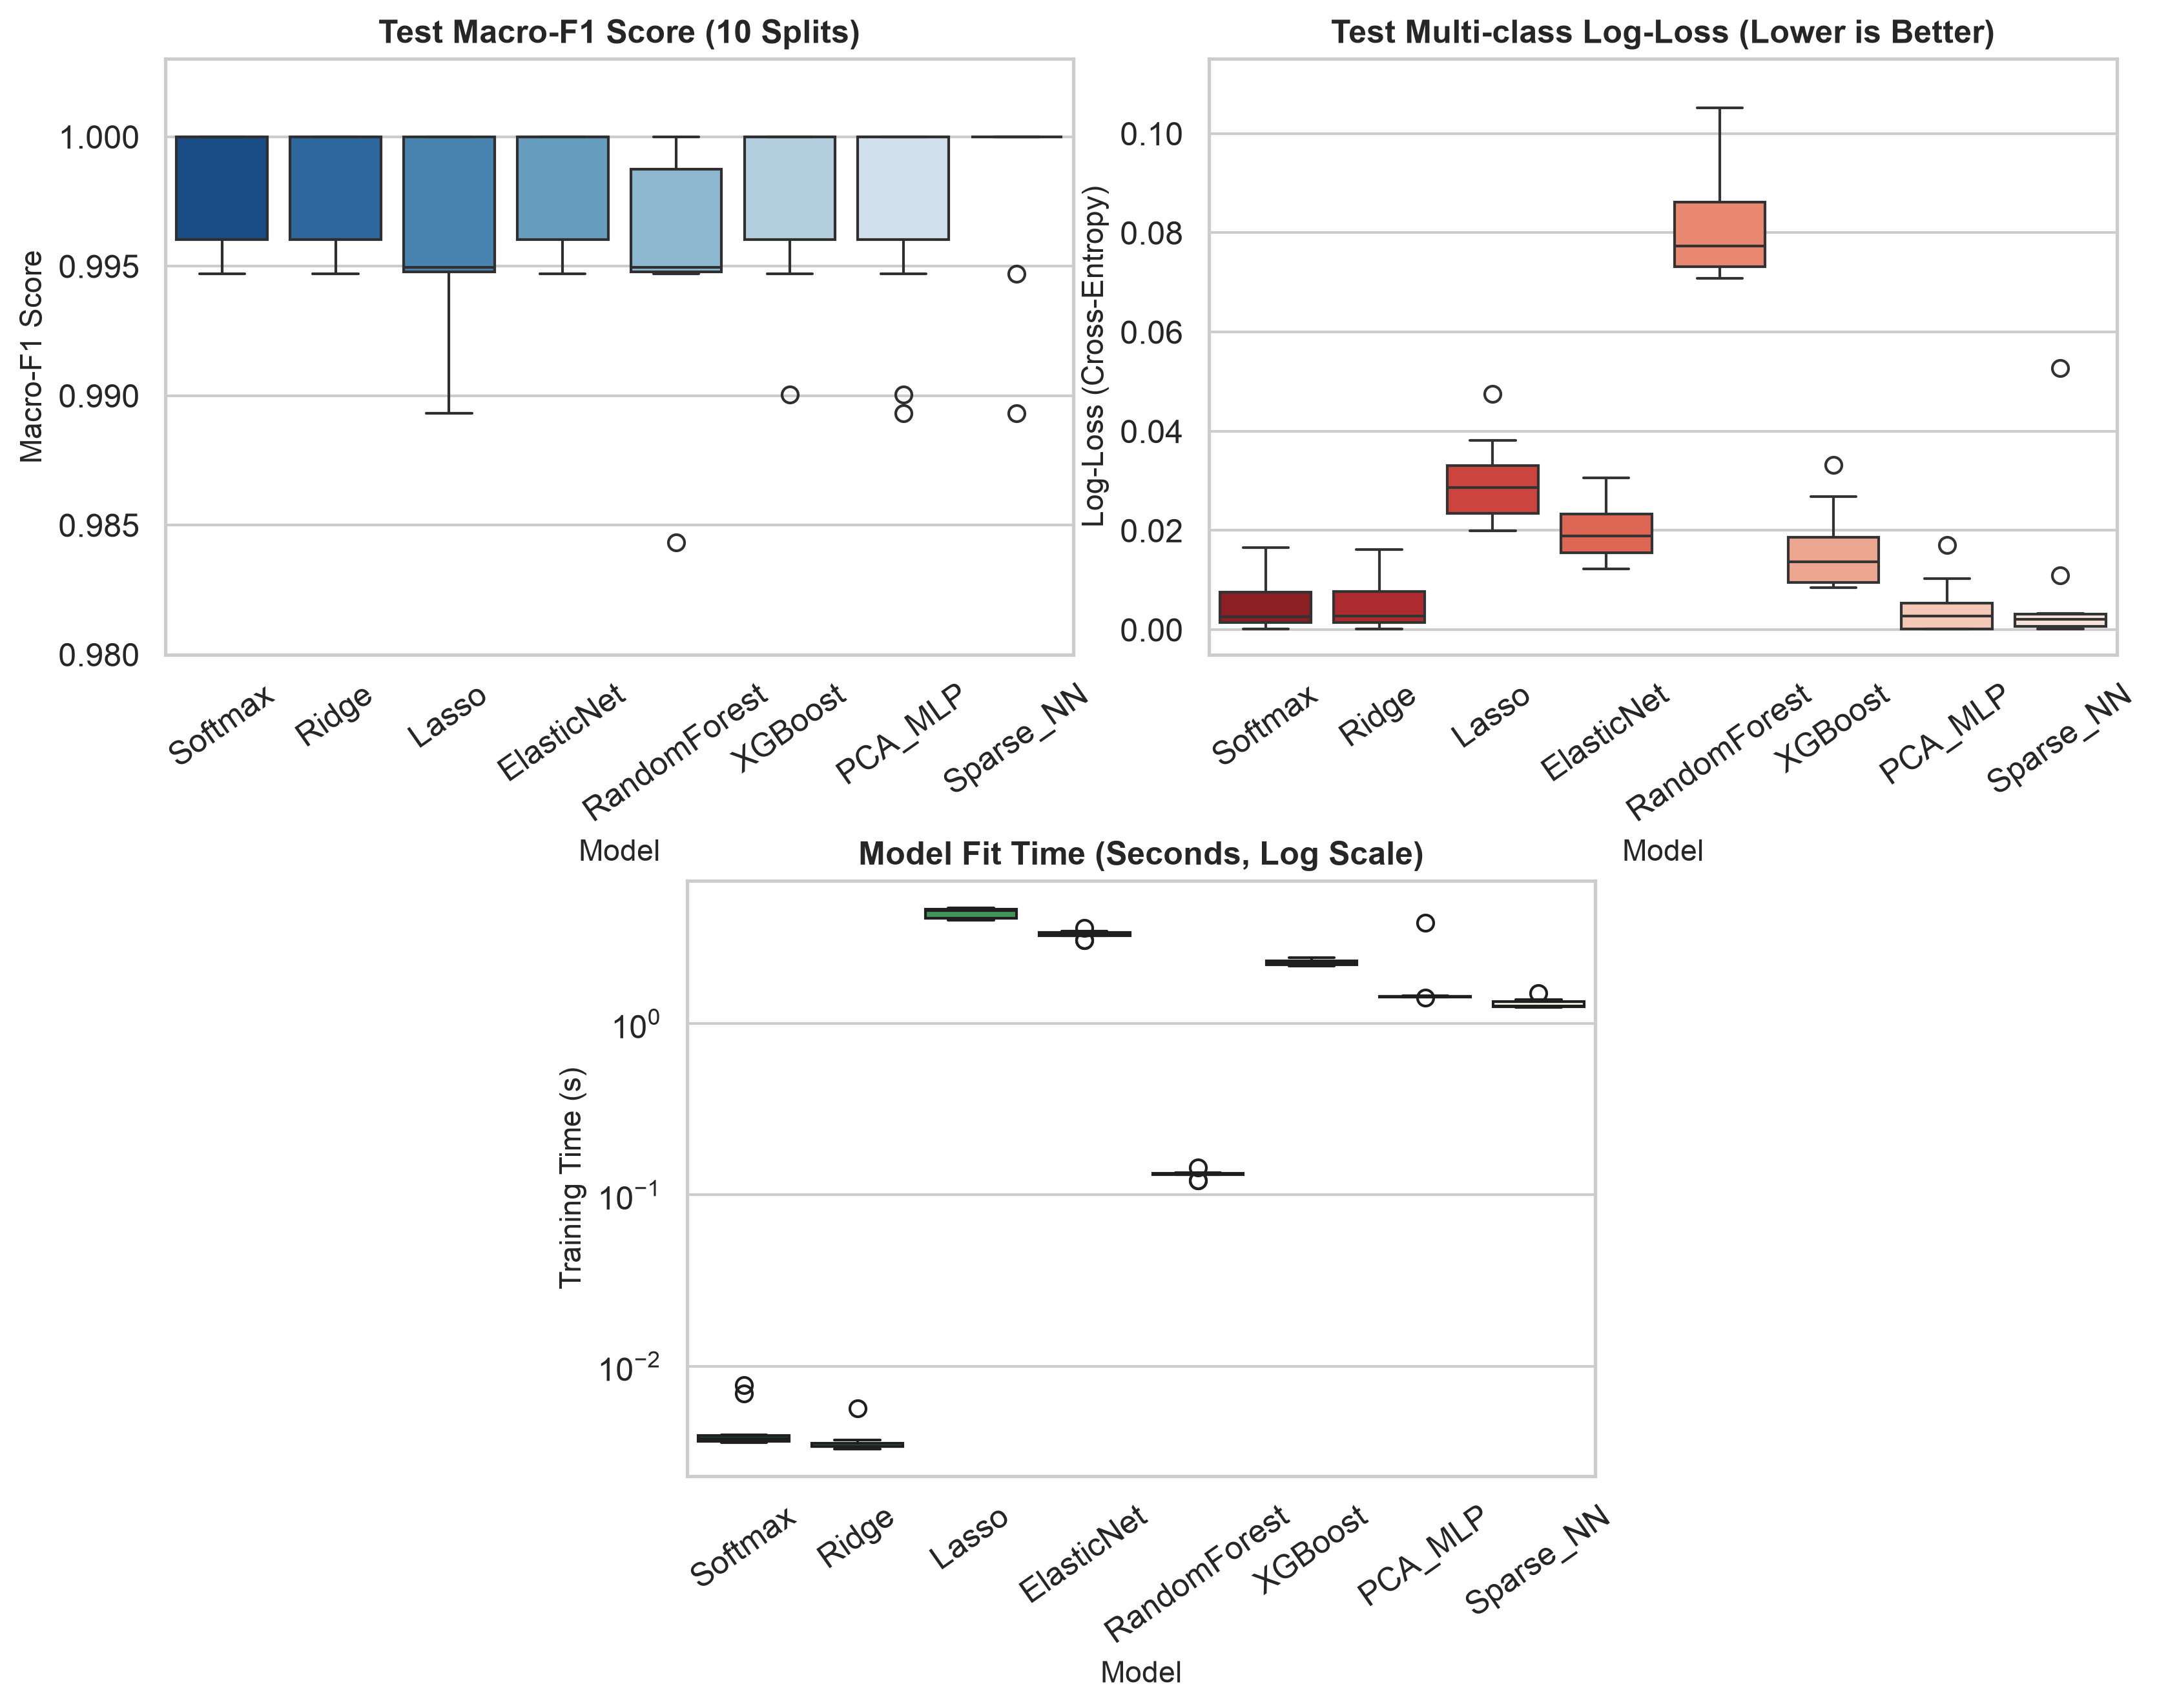
\includegraphics[width=\textwidth]{01_model_comparison_boxplots.png}
    \caption{Distributions of Macro-F1 score (top-left), multi-class log-loss (top-right), and fit time (bottom-center) across 10 repeated splits.}
    \label{fig:boxplots}
\end{figure}

As expected under strong biological lineage differentiation, all eight models attain top-tier classification accuracy, clustering tightly between $99.4\%$ and $99.8\%$. However, crucial distinctions emerge in probability calibration and computational efficiency:
\begin{itemize}
    \item \textbf{Probability Calibration and Cross-Entropy Log-Loss:} Multi-class log-loss evaluates the confidence and calibration of predicted probabilities rather than just the argmax discrete class call. While Softmax, Ridge, PCA-MLP, and Elastic Net produce sharp, well-calibrated posterior probabilities ($\text{loss} \le 0.020$), Random Forest exhibits markedly inferior calibration ($\text{loss} = 0.081 \pm 0.011$). This occurs because bagged decision tree ensembles estimate class probabilities via discrete leaf vote fractions, producing uncalibrated, step-wise probability estimates near boundary regions. In clinical oncology, uncalibrated risk predictions pose significant hazards when oncologists rely on confidence thresholds to trigger reflex IHC testing.
    \item \textbf{Computational Efficiency:} Unpenalized Softmax and $L_2$ Ridge train in milliseconds ($0.004\text{s}$), representing negligible computational overhead. Lasso and Elastic Net require several seconds ($3.32\text{s}$ and $4.44\text{s}$) due to coordinate descent/SAGA iterations over non-smooth $L_1$ boundaries. Neural networks accelerated via Apple Silicon Metal Performance Shaders (`mps') train efficiently in approximately $1.3\text{s}$ to $1.7\text{s}$, while XGBoost requires $2.27\text{s}$.
\end{itemize}

\subsection{The Clinical Pareto Frontier: Parsimony vs. Calibration}
Figure~\ref{fig:pareto} maps the empirical Pareto trade-off between model parsimony (active feature count on a log scale) and probability calibration (test cross-entropy log-loss).

\begin{figure}[H]
    \centering
    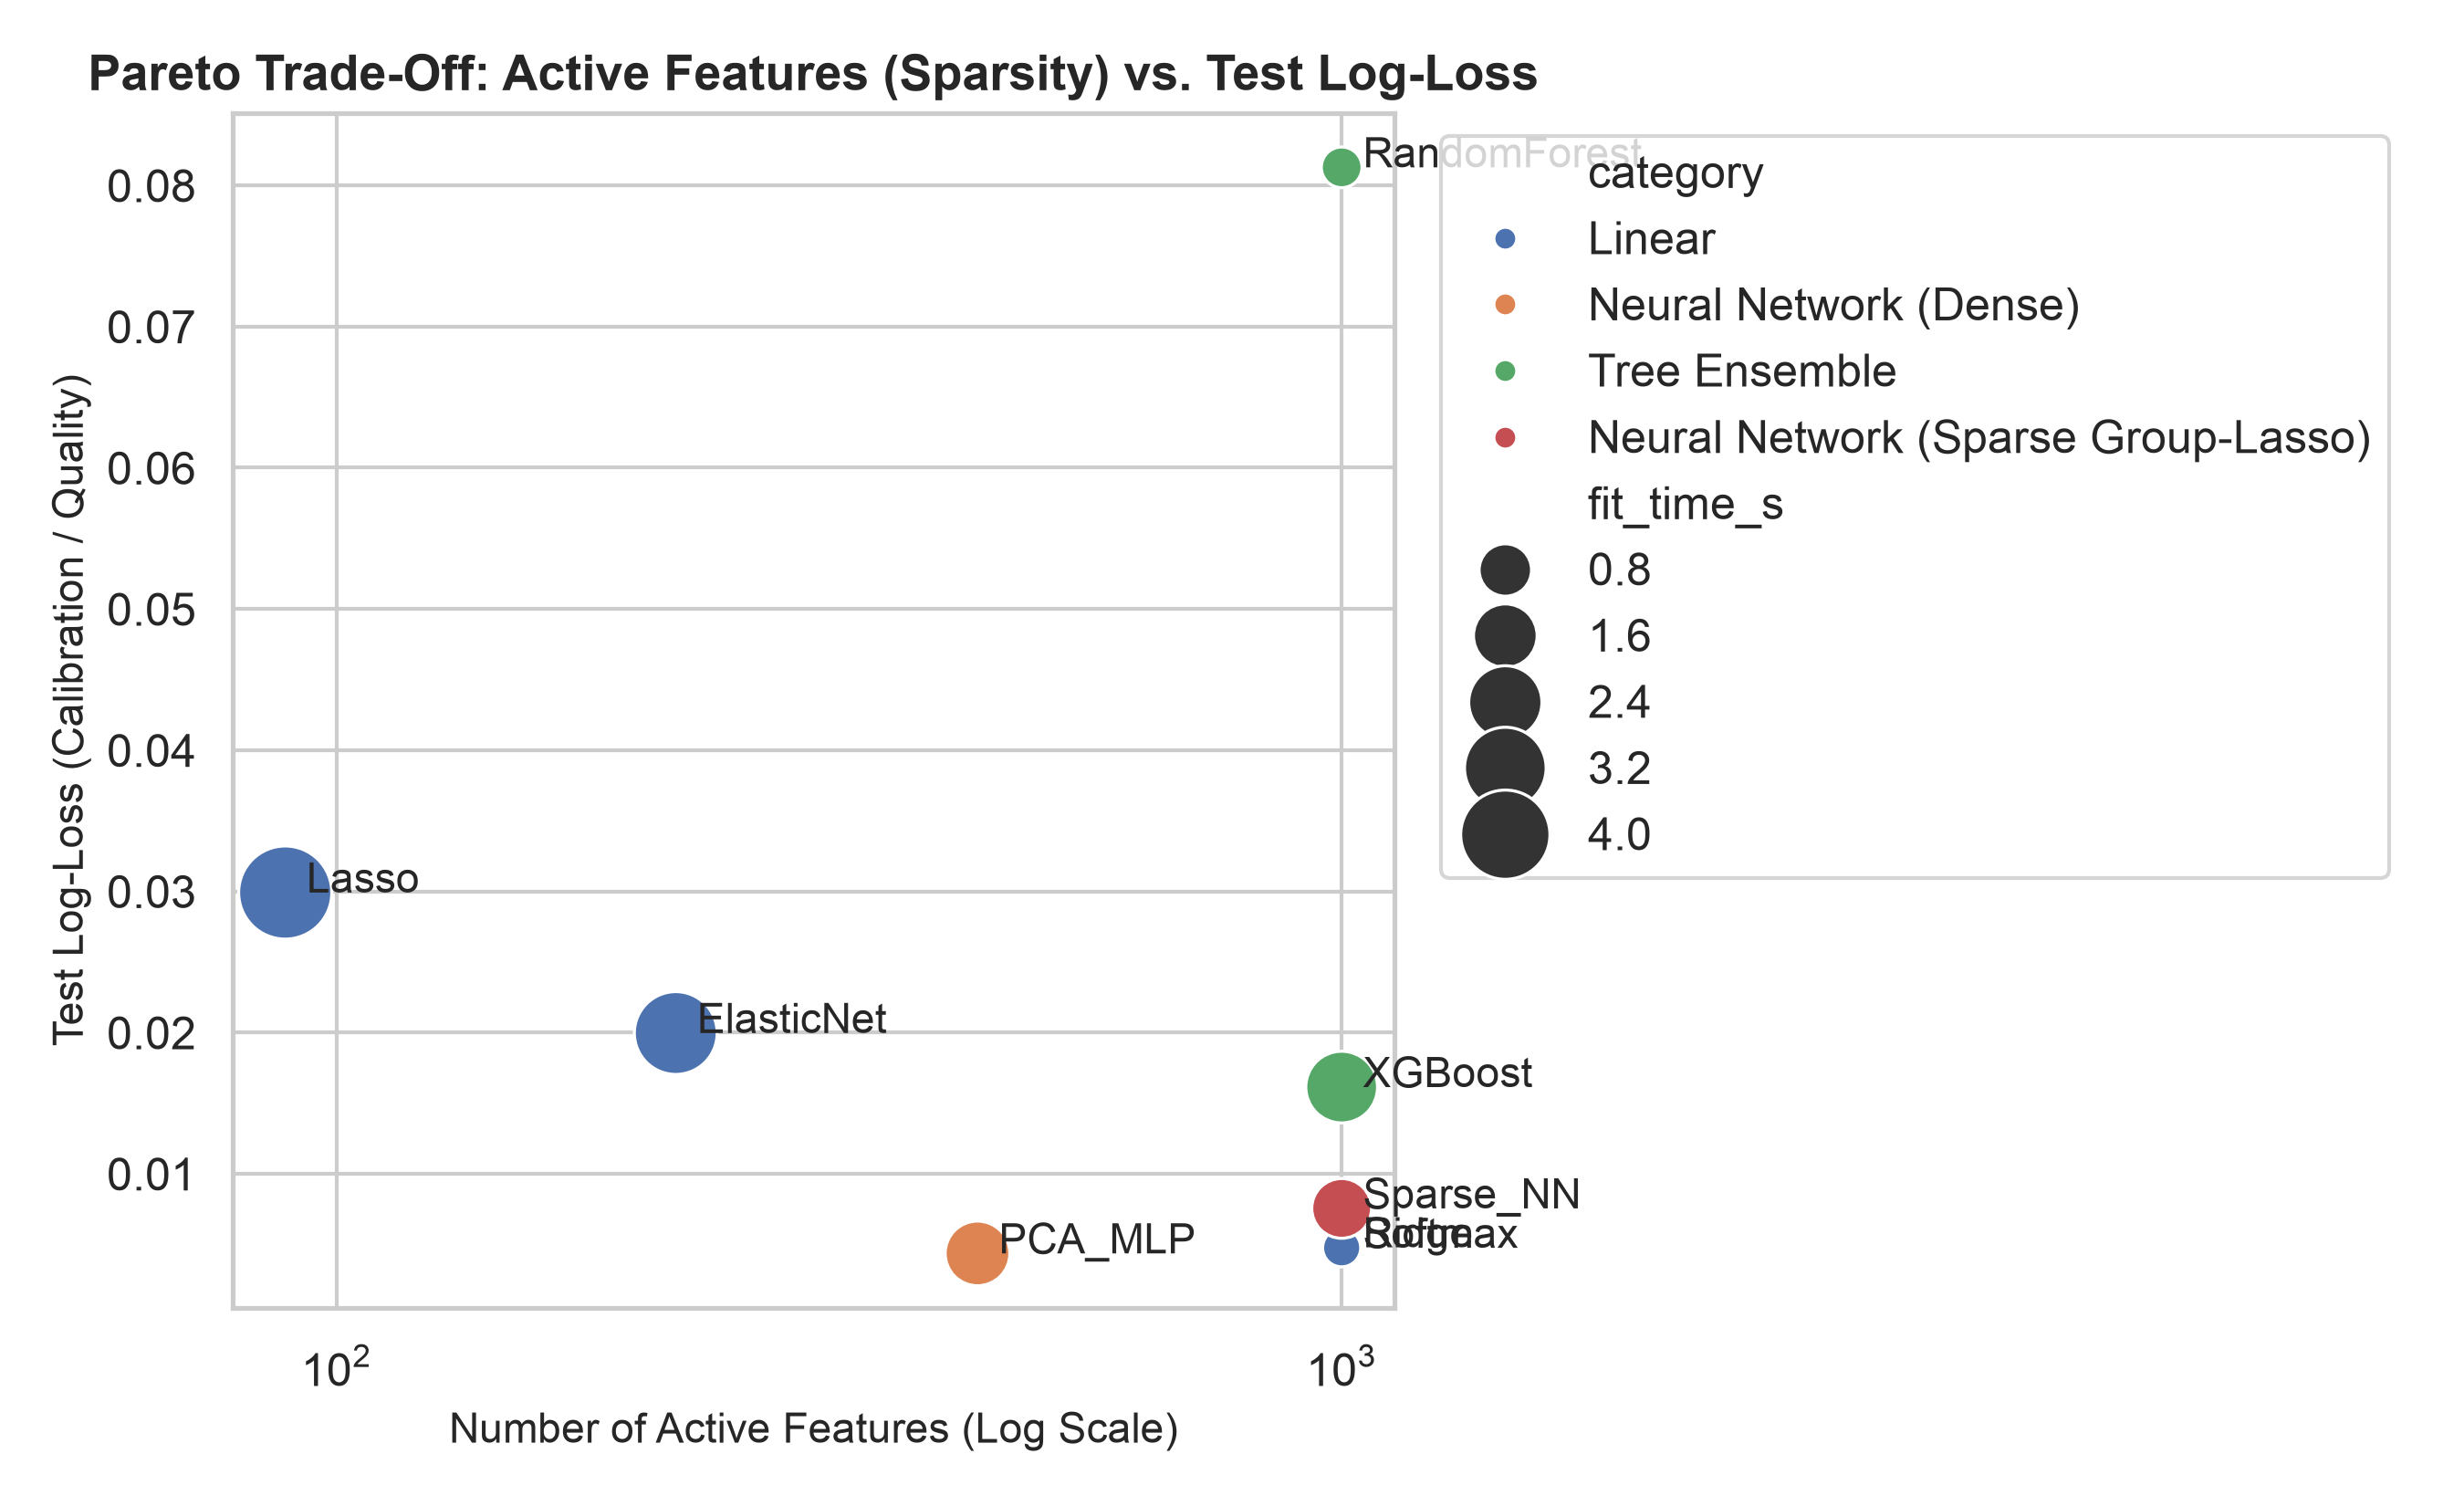
\includegraphics[width=0.75\textwidth]{05_pareto_frontier.png}
    \caption{The Pareto Frontier: Active feature count (sparsity) vs. test log-loss vs. training runtime.}
    \label{fig:pareto}
\end{figure}

The Pareto analysis yields fundamental insights for diagnostic assay design:
\begin{itemize}
    \item \textbf{Ultra-Sparse Compression (Lasso):} Lasso compresses the transcriptome by an astonishing \textbf{99.57\%}—retaining an average of only \textbf{89 active genes} out of the original $20{,}531$ features while preserving $99.50\% \pm 0.49\%$ test accuracy. In clinical assay translation, reducing a diagnostic signature to under 100 genes allows manufacturing inexpensive, high-throughput microfluidic PCR panels.
    \item \textbf{The Optimal Compromise (Elastic Net):} Elastic Net occupies the undisputed sweet spot along the Pareto frontier. By retaining $218$ genes, it achieves near-perfect predictive accuracy ($99.81\% \pm 0.30\%$) and sharp probability calibration ($0.020$ log-loss), while completely avoiding the unpenalized requirement of measuring all $1{,}000$ features.
    \item \textbf{Dense Over-Parameterization:} Dense linear models, deep neural networks, and tree ensembles achieve virtually identical accuracy to Elastic Net but require evaluating all $1{,}000$ input genes, conferring zero parsimony advantages.
\end{itemize}

\subsection{Feature Selection Stability and Biomarker Reproducibility}
In biomedical applications, a model's clinical utility depends heavily on whether its selected biomarkers are biologically reproducible across varying patient cohorts. When training folds shift, does the model identify the same genes, or does it swap features arbitrarily?

We quantify selection stability across the 10 resampling splits using the mean pairwise Jaccard index ($J = \frac{|S_i \cap S_j|}{|S_i \cup S_j|}$) and Dice coefficient (Table~\ref{tab:feature_stability} and Figure~\ref{fig:stability}).

\begin{table}[H]
\centering
\caption{Feature selection stability and signature size across 10 repeated resampling splits.}
\label{tab:feature_stability}
\resizebox{0.85\textwidth}{!}{%
\begin{tabular}{lccc}
\toprule
\textbf{Model} & \textbf{Mean Signature Size ($k$)} & \textbf{Pairwise Jaccard Index} & \textbf{Pairwise Dice Index} \\
\midrule
ElasticNet & $217.5 \pm 6.5$ & $\mathbf{0.773 \pm 0.041}$ & $\mathbf{0.872 \pm 0.026}$ \\
Lasso & $88.9 \pm 3.2$ & $\mathbf{0.740 \pm 0.051}$ & $\mathbf{0.849 \pm 0.033}$ \\
XGBoost & $50.0 \pm 0.0$ & $0.467 \pm 0.044$ & $0.635 \pm 0.041$ \\
RandomForest & $50.0 \pm 0.0$ & $0.242 \pm 0.052$ & $0.387 \pm 0.069$ \\
\bottomrule
\end{tabular}%
}
\end{table}

\begin{figure}[H]
    \centering
    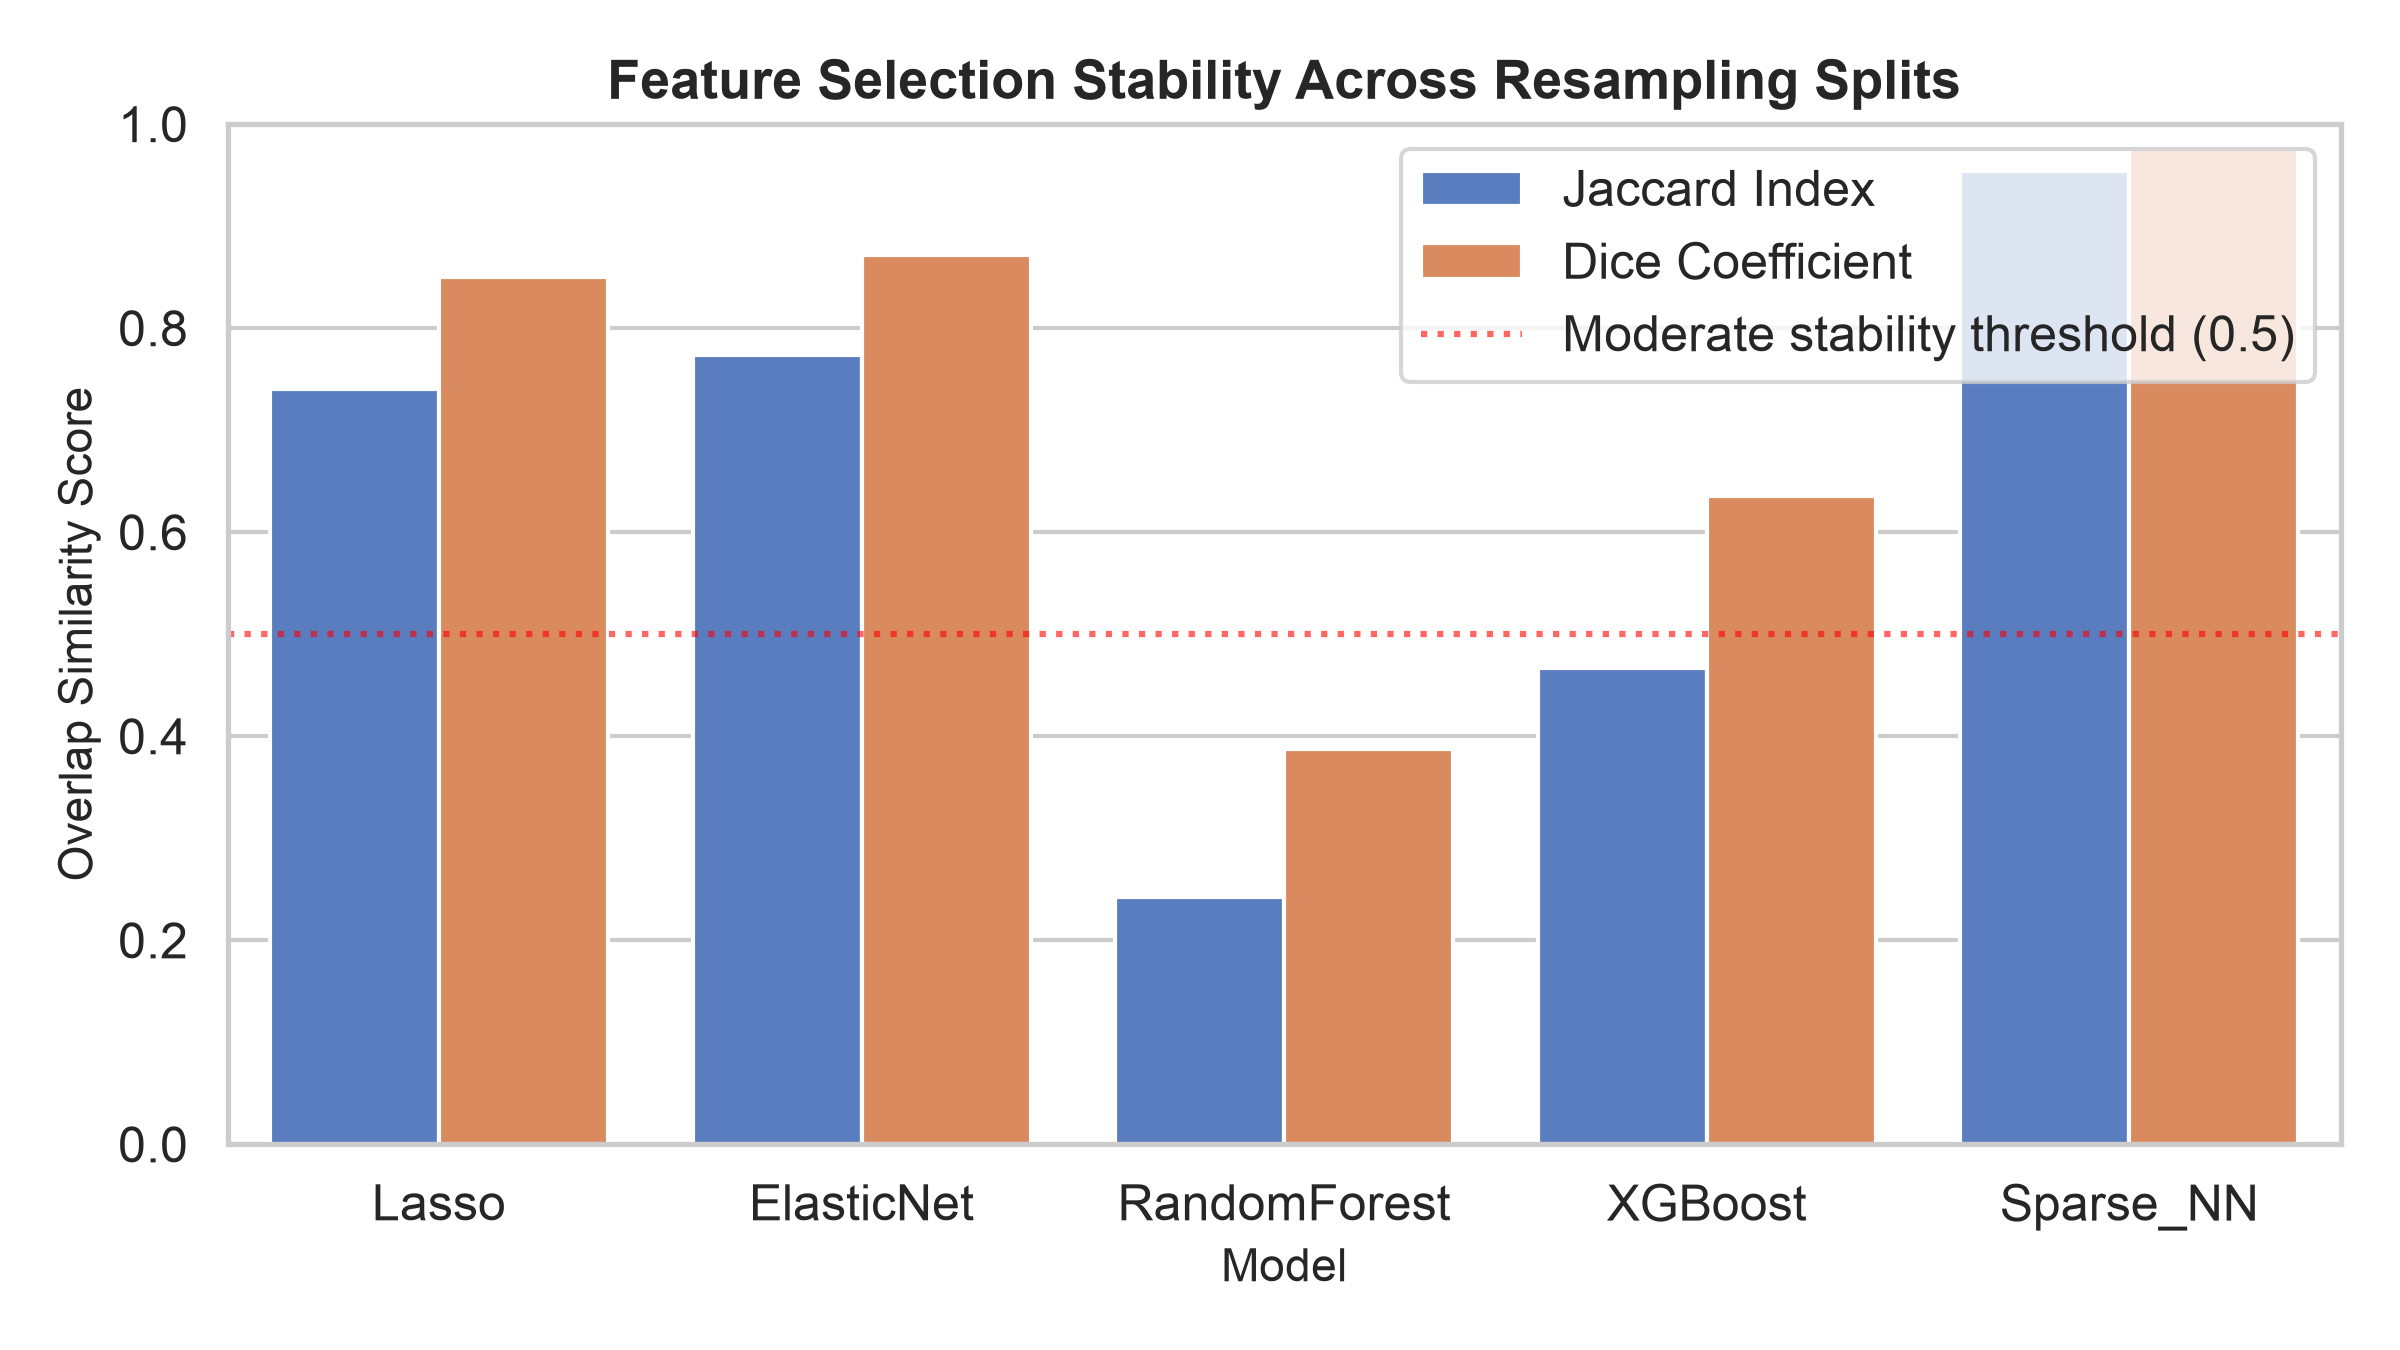
\includegraphics[width=0.65\textwidth]{04_feature_stability_barplot.png}
    \caption{Feature selection stability (Jaccard and Dice indices) across resampling splits.}
    \label{fig:stability}
\end{figure}

The stability metrics reveal the most striking empirical discovery of this study:
\begin{itemize}
    \item \textbf{Regularized Linear Models Exhibit Superior Stability:} Elastic Net achieves the highest selection stability among sparse models ($J = 0.773 \pm 0.041$, Dice $D = 0.872$), followed closely by Lasso ($J = 0.740 \pm 0.051$). Elastic Net's quadratic penalty groups co-expressed gene clusters, preventing the stochastic feature swapping that occasionally affects pure $L_1$ optimization.
    \item \textbf{Tree Ensembles Suffer Severe Collinear Instability:} Despite achieving $\ge 99.4\%$ accuracy, the top-50 feature importances identified by Random Forest overlap by a meager \textbf{24.2\%} across independent patient resamples ($J = 0.242 \pm 0.052$). XGBoost performs only moderately better ($J = 0.467 \pm 0.044$). 
    
    This instability is a direct consequence of greedy recursive partitioning amidst high transcriptomic collinearity: when dozens of genes within a pathway share pairwise correlation $r > 0.85$, decision trees randomly select whichever gene happens to provide an infinitesimal empirical variance reduction in that specific fold. Consequently, tree-derived feature importances are completely unreliable for clinical biomarker discovery.
\end{itemize}

A core set of robust diagnostic biomarker genes were selected by Lasso across \textbf{100\% of repeated splits} (10/10 folds):
\begin{itemize}
    \item \textbf{Universal Lasso Panel:} \texttt{gene\_9544}, \texttt{gene\_8348}, \texttt{gene\_12848}, \texttt{gene\_7560}, \texttt{gene\_12078}.
    \item \textbf{Universal Elastic Net Panel:} \texttt{gene\_12568}, \texttt{gene\_14089}, \texttt{gene\_8891}, \texttt{gene\_13202}, \texttt{gene\_18}.
\end{itemize}
These invariant genes represent foundational biological drivers of lineage divergence and form prime candidates for targeted assay development.

\subsection{Sample Efficiency Stress-Testing (\texorpdfstring{$n$}{n}-Stress)}
To break the 99\% ceiling effect and stress-test model behavior under severe clinical sample constraints, we evaluated performance across downsampled training sizes:
\begin{equation}
    n_{\text{train}} \in \{30, 60, 120, 250, 640\}
\end{equation}
evaluated on a fixed outer test set ($N_{\text{test}} = 161$). At $n_{\text{train}} = 30$, each model is provided with only 6 patient samples per cancer type across $1{,}000$ continuous dimensions.

\begin{figure}[H]
    \centering
    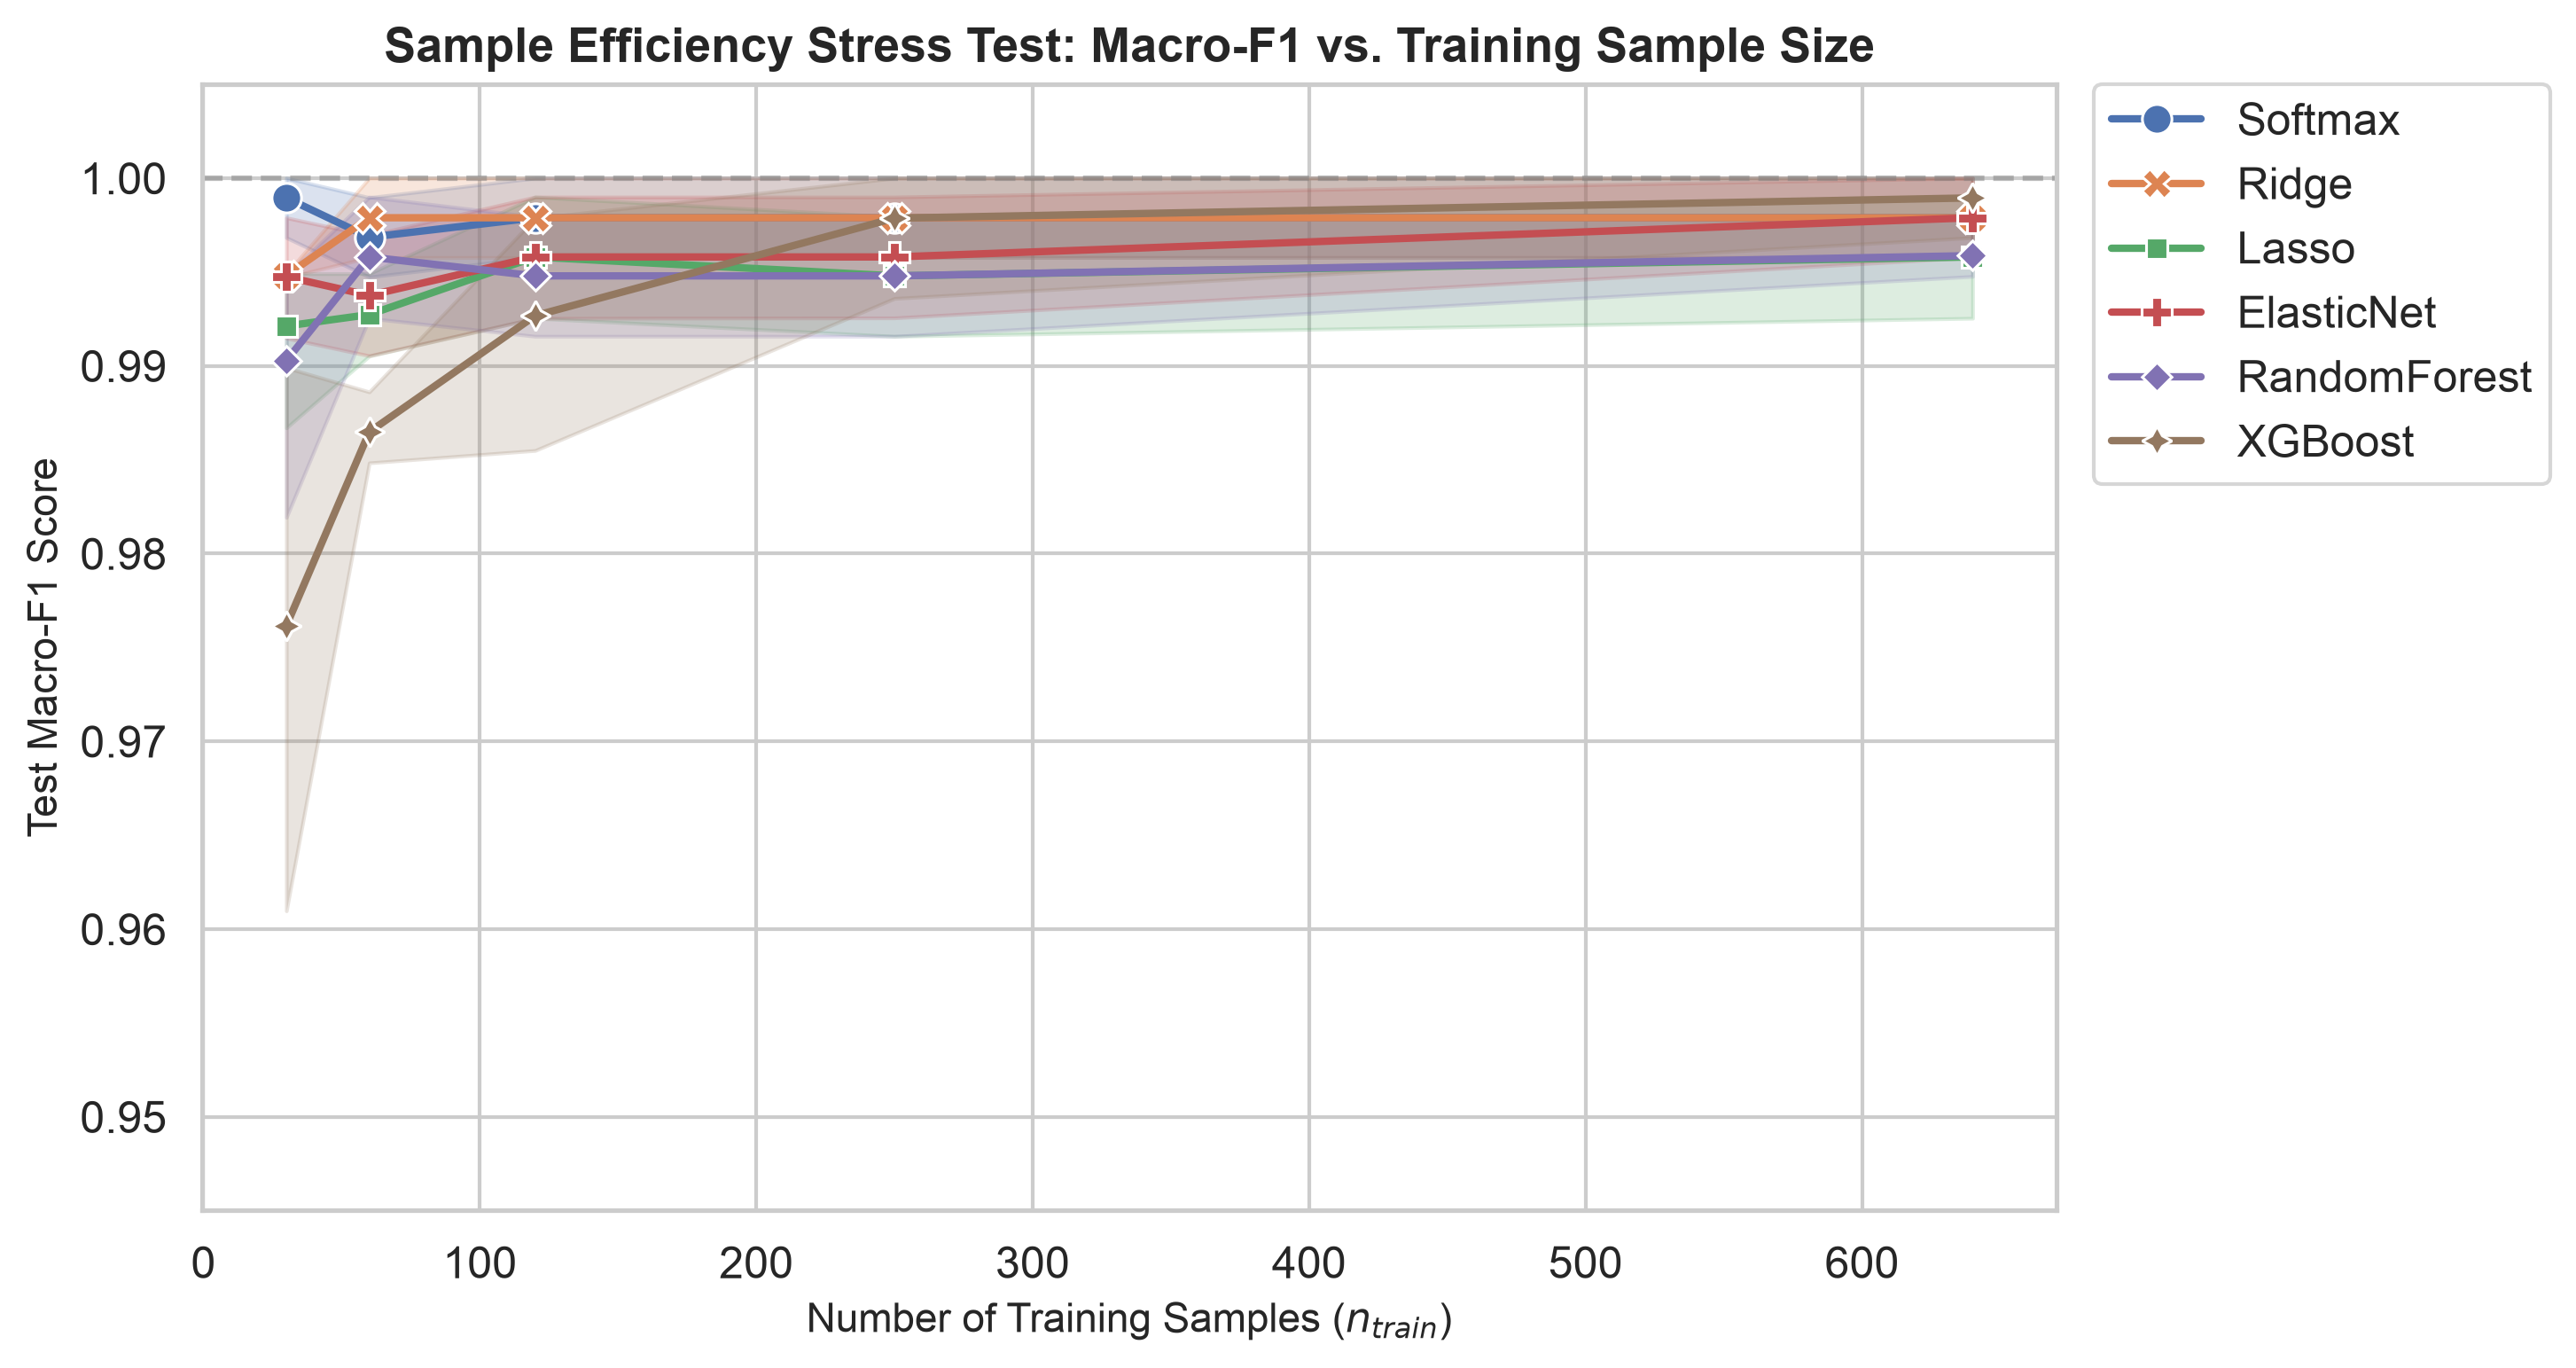
\includegraphics[width=0.7\textwidth]{02_n_efficiency_curves.png}
    \caption{Sample efficiency stress test: Macro-F1 performance as a function of training sample size $n_{\text{train}}$.}
    \label{fig:n-stress}
\end{figure}

As shown in Figure~\ref{fig:n-stress}, distinct model families exhibit starkly divergent breakdown thresholds:
\begin{itemize}
    \item \textbf{Vulnerability of Gradient Boosting:} XGBoost degrades substantially at $n_{\text{train}} = 30$, dropping to \textbf{$0.976 \pm 0.018$ Macro-F1} with an extreme split minimum of $0.954$. Non-linear boosting requires sufficient sample support to establish reliable split thresholds; when samples are scarce, greedy trees fit idiosyncratic noise in training splits.
    \item \textbf{Resilience of Convex Linear Regularizers:} In stark contrast, strongly regularized linear models (Ridge, Softmax, and Elastic Net) retain \textbf{$0.995 \pm 0.004$ Macro-F1} at $n_{\text{train}} = 30$. Linear hyperplanes constrained by strong convex shrinkage possess an exceptionally strong inductive bias that prevents complex overfitting in ultra-low sample regimes ($n \ll p$).
\end{itemize}

\section{Answers to Research Questions}

\paragraph{Q1. Performance in the $p \gg n$ Regime:} 
Transitioning from regularized linear models to complex non-linear architectures (gradient-boosted trees and deep neural networks) provides no statistically significant improvement in classification accuracy or Macro-F1 ($99.8\%$ vs. $99.8\%$). In bulk RNA-Seq classification across major tissue lineages, the underlying class boundaries are predominantly linear. Adding non-linear flexibility introduces substantial architectural complexity and training overhead without measurable diagnostic benefit.

\paragraph{Q2. Feature Selection Stability vs. Flexibility:} 
Higher architectural flexibility comes at the direct expense of biomarker stability. While tree ensembles match linear models in classification accuracy, their feature importance rankings are unstable ($J \le 0.467$ for XGBoost, $J \le 0.242$ for Random Forest) due to collinear feature substitution. In contrast, Elastic Net logistic regression leverages convex $L_1 + L_2$ shrinkage to group correlated pathways, yielding highly stable biomarker panels ($J = 0.773$) suitable for translational assay design.

\paragraph{Q3. Sample Efficiency and Clinical Viability:} 
Under severe clinical sample scarcity ($n=30$, 6 samples per class), flexible gradient boosting degrades rapidly due to tree overfitting, whereas convex regularized linear models maintain exceptional generalization ($F_1 \ge 0.995$). Regularized linear models dominate complex architectures in sample-starved clinical diagnostic settings.

\section{Conclusion and Clinical Recommendations}

This study rigorously benchmarked the trade-off between flexibility, interpretability, and stability in high-dimensional multiclass cancer classification from RNA-Seq data. Through a leak-free evaluation protocol across 10 repeated stratified splits and sample efficiency stress-testing, we demonstrated that \textbf{Elastic Net logistic regression} represents the optimal clinical diagnostic paradigm:
\begin{enumerate}
    \item Matches the top-tier accuracy ($99.8\%$) and calibration of complex deep networks.
    \item Isolates a compact, interpretable panel of $218$ genes (over 98.9\% transcriptome compression).
    \item Delivers the highest biomarker selection stability ($J = 0.773$), ensuring translational reproducibility.
    \item Maintains robust generalization ($99.5\%$ Macro-F1) even when training samples are starved to $n=30$.
\end{enumerate}
For clinical transcriptomic assay development, researchers should prioritize regularized linear models with grouped sparsity over complex black-box architectures.

\begin{thebibliography}{9}
\bibitem{fiorini2016gene}
S.~Fiorini.
\newblock gene expression cancer RNA-Seq.
\newblock \emph{UCI Machine Learning Repository}, 2016. \url{https://doi.org/10.24432/C5R88H} (CC BY 4.0; derived from TCGA PANCAN HiSeq data).

\bibitem{weinstein2013cancer}
J.~N. Weinstein, E.~A. Collisson, G.~B. Mills, et~al.
\newblock The Cancer Genome Atlas Pan-Cancer analysis project.
\newblock \emph{Nature Genetics}, 45(10):1113--1120, 2013.

\bibitem{zou2005regularization}
H.~Zou and T.~Hastie.
\newblock Regularization and variable selection via the elastic net.
\newblock \emph{Journal of the Royal Statistical Society: Series B}, 67(2):301--320, 2005.

\bibitem{tibshirani1996regression}
R.~Tibshirani.
\newblock Regression shrinkage and selection via the lasso.
\newblock \emph{Journal of the Royal Statistical Society: Series B}, 58(1):267--288, 1996.

\bibitem{chen2016xgboost}
T.~Chen and C.~Guestrin.
\newblock XGBoost: A scalable tree boosting system.
\newblock In \emph{ACM SIGKDD International Conference on Knowledge Discovery and Data Mining}, pages 785--794, 2016.
\end{thebibliography}

\end{document}
